\documentclass[12pt]{article}
\usepackage{amsmath}
\usepackage{graphicx}
\usepackage{hyperref}
\usepackage[utf8]{inputenc}
\usepackage{geometry}
\usepackage{mathtools}
\usepackage{empheq}
\usepackage{listings}
\usepackage{xcolor}
\usepackage{caption}
\usepackage{subcaption}
\usepackage{setspace}
\usepackage{indentfirst}
\usepackage{authblk}
\usepackage{svg}

\graphicspath{ {./assets/} }
\geometry{margin=1in}
\doublespacing
\captionsetup{labelfont=bf}

\title{CHEN 425 Workshop 1}
\author{Mark Levchenko}
\date{25 January 2023}

\begin{document}

% \maketitle

% \par\noindent\rule{\textwidth}{0.4pt}

\textbf{CHEN 425 ASPEN Simulation Report}

\textbf{Title:} Simulation of a Flash Process

\textbf{Workshop:} \#2

\textbf{Date:} February 15, 2023

\textbf{Prepared by:} Mark Levchenko

\textbf{To:} Professor Mahmoud El-Halwagi

\section{Summary of Results}

\begin{enumerate}
    \item Vapor flow: 32290.72 kmol/hr

    Vapor stream composition:

    \begin{tabular}{|c c|}
         \hline
         Species & Mole fraction \\
         \hline
            HYDROGEN & 0.272523897 \\
            CO & 0.148649452 \\
            N2 & 0.421173402 \\
            WATER & 0.009009942 \\
            CO2 & 0.061931519 \\ 
            METHANE & 0.049549613 \\
            ETHYLENE & 0.02477473 \\
            CYCLOHEXANE & 0.012387445 \\
         \hline
    \end{tabular}

    \item Heat curve:

    \includesvg[scale=0.9]{heat_curve.svg}

    The dew point is 273.61 $^\circ$F.

    \item A temperature of 240 $^\circ$F is required for the overall vapor fraction to be 90\%.
\end{enumerate}

\section{Discussion of Simulation Results}

\begin{enumerate}
    \item Stream results for part i:

    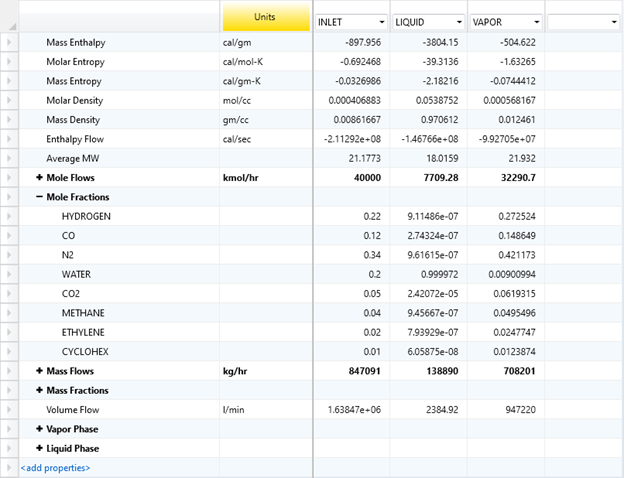
\includegraphics[scale=0.9]{parti.png}

    \item ASPEN Heat Curve:

    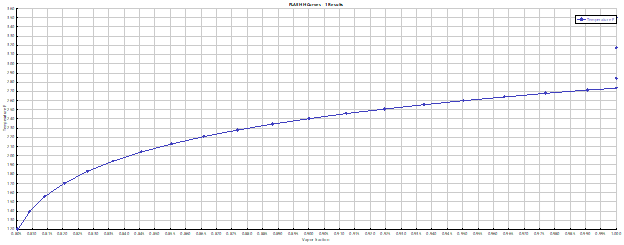
\includegraphics[scale=0.9]{curve.png}

    The dew point is the temperature at which the vapor fraction changes to 1. ASPEN reports this point in the results.

    \item Stream results showing that the vapor stream is 90\% of the overall flow rate.

    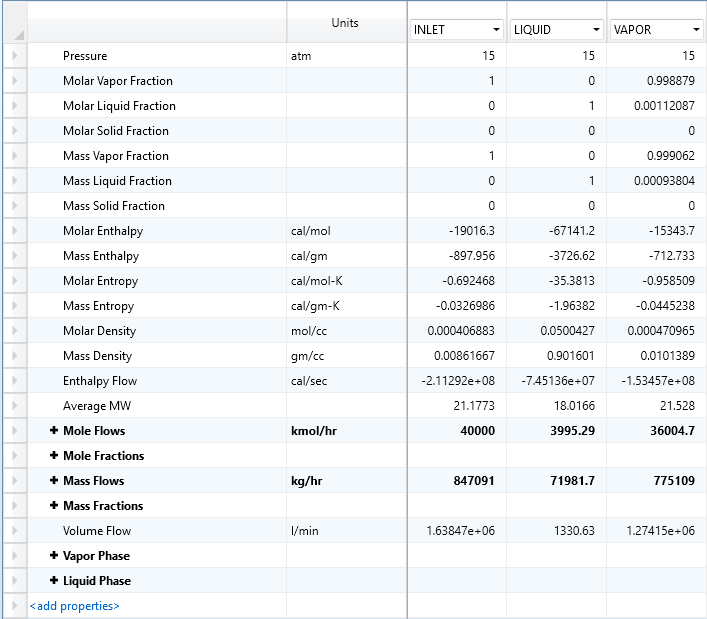
\includegraphics[scale=0.8]{partiii.png}

    Find on the heat curve where the vapor fraction is 0.9, and find the corresponding temperature.

\end{enumerate}

\section{Simulation Screenshots}

Main flowsheet:

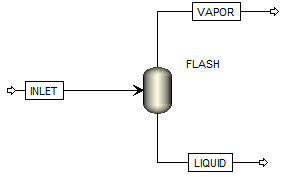
\includegraphics{flowsheet.png}

Stream results are included in the discussion section. 


\section{Conclusions}

\begin{enumerate}
    \item It looks like the vapor is more concentrated in the more volatile components than the feed. The vapor flow is the majority of the outlet flow.

    \item Looking at the heat curve, it is clear where the vapor becomes saturated. Above the dew point, the vapor fraction is constant.

    \item The vapor fraction increases as the temperature increases. This increase can be seen in the heat curve and by comparing the results bewteen part i and part iii.
\end{enumerate}


\end{document}